\documentclass[12pt, letterpaper, preprint]{aastex}
\usepackage[breaklinks,colorlinks, urlcolor=blue,citecolor=blue,linkcolor=blue]{hyperref}
\usepackage{color}
\usepackage{bm}
%%% This file is generated by the Makefile.
\newcommand{\giturl}{\url{https://github.com/changhoonhahn/nonGaussLike}}
\newcommand{\githash}{0cff07b}\newcommand{\gitdate}{2018-01-09}\newcommand{\gitauthor}{ChangHoon Hahn}


% typesetting shih
\linespread{1.08} % close to 10/13 spacing
\setlength{\parindent}{1.08\baselineskip} % Bringhurst
\setlength{\parskip}{0ex}
\let\oldbibliography\thebibliography % killin' me.
\renewcommand{\thebibliography}[1]{%
  \oldbibliography{#1}%
  \setlength{\itemsep}{0pt}%
  \setlength{\parsep}{0pt}%
  \setlength{\parskip}{0pt}%
  \setlength{\bibsep}{0ex}
  \raggedright
}
\setlength{\footnotesep}{0ex} % seriously?

% citation alias
\defcitealias{beutler2017}{B2017}
\defcitealias{sinha2017a}{S2017}

% math shih
\newcommand{\setof}[1]{\left\{{#1}\right\}}
\newcommand{\given}{\,|\,}
\newcommand{\pseudo}{{\mathrm{pseudo}}}
\newcommand{\Var}{\mathrm{Var}}
% text shih
\newcommand{\foreign}[1]{\textsl{#1}}
\newcommand{\etal}{\foreign{et~al.}}
\newcommand{\opcit}{\foreign{Op.~cit.}}
\newcommand{\documentname}{\textsl{Article}}
\newcommand{\equationname}{equation}
\newcommand{\bitem}{\begin{itemize}}
\newcommand{\eitem}{\end{itemize}}
\newcommand{\beq}{\begin{equation}}
\newcommand{\eeq}{\end{equation}}
\newcommand{\todo}[1]{{\bf \textcolor{red}{#1}}}
\newcommand{\Dmock}{{\bf D}^\mathrm{mock}}
\newcommand{\Xmock}{{\bf X}^\mathrm{mock}}
\newcommand{\Xref}{{\bf X}^\mathrm{ref}}
\newcommand{\Yref}{{\bf Y}^\mathrm{ref}}
\newcommand{\Ralpha}{R\'enyi-$\alpha$}
\newcommand{\Beut}{\citetalias{beutler2017}}
\newcommand{\Sinh}{\citetalias{sinha2017a}}

\newcommand{\patchy}{{\fontshape\scdefault\selectfont patchy}}

\begin{document}\sloppy\sloppypar\frenchspacing 

%\title{How I Learned to Stop Worrying and Love The Central Limit Theorem}
\title{Likelihood Non-Gaussianity in Large Scale Structure Analyses}
\date{\texttt{DRAFT~---~\githash~---~\gitdate~---~NOT READY FOR DISTRIBUTION}}
\author{ChangHoon~Hahn\refstepcounter{footnote}\refstepcounter{footnote}, et al.} %Florian~Beutler, Manodeep~Sinha, Andreas~Berlind}
\affil{Lawrence Berkeley National Laboratory, 1 Cyclotron Rd, Berkeley CA 94720, USA}
\email{changhoon.hahn@lbl.gov}

\begin{abstract}
    abstract here 
\end{abstract}

\keywords{
methods: statistical
---
galaxies: statistics
---
methods: data analysis
---
cosmological parameters
---
cosmology: observations
---
large-scale structure of universe
}

\section{Introduction}
\begin{itemize}
    \item Talk about the use of Bayesian parameter inference and getting the posterior in LSS cosmology 
    \item Explain the two major assumptions that go into evaluating the likelihood
    \item Emphasize that we are not talking about non-Gaussian contributions to the likelihood
    \item Emphasize the scope of this paper is to address whether one of the assumptions matters for 
        galaxy clustering analyses. 
\end{itemize}

\section{Gaussian Likelihood Assumption} \label{sec:gaussass} 
\begin{itemize}
    \item Depending on Hogg's paper maybe a simple illustration of how the likelihood asumption 
\end{itemize}

\todo{However, as we show in this paper, the assumption of likelihood 
Gaussianity is not necessary. In fact, we will show that the mock catalogs 
used in standard LSS analyses to estimate the covariance matrix for 
evaluating the Gaussian likelihood, can be used to quantify the non-Gaussianity. 
More important the mock catalogs can be used to construct an accurate 
estimator for the non-Gaussian likelihood.} 

\section{Mock Catalogs}
Mock catalogs are play an indispensable role in standard cosmological 
anslyses of LSS studies. They're used for testing analysis 
pipelines~\citep[][]{beutler2017, grieb2017, tinkerinpreparation}, 
testing the effect of systematics~\citep{guo2012, vargas-magana2014, hahn2017, pinol2017, ross2017}, 
and, most relevantly for this paper, estimating the covariance 
matrix~\citep[][]{parkinson2012, kazin2014, grieb2017, alam2017, beutler2017, sinha2017a}. 
In fact, nearly all current state-of-the-art LSS analyses use
covariance matrices estimated from mocks to evaluate the likelihood 
for parameter inference. 

While some argue for analytic estimates of the covariance 
matrix~\citep[e.g.][]{mohammed2017} or estimates directly from data
by subsampling~\citep[e.g.][]{norberg2009}, covariance matrices 
from mocks have a number of advantages. Mock catalogs allow us 
to incorporate detailed systematic errors present in the 
data and variance beyond the volume of the data. Even for analytic 
estimates, large ensembles of mocks are crucial for validataion~\citep{slepian2017}. 
Moreover, as we show later in this paper, mock catalogs present an
additional advantage: they allow us to 
quantify the non-Gaussianity of the likelihood and more accurately 
estimate the true likelihood. 

In this paper, we we focus on two LSS analyses: the powerspectrum 
multipole full shape analysis of \cite{beutler2017} and group multiplicity 
function analysis of \cite{sinha2017a}. Throughout the paper we will 
make extensive use of the mock catalogs used in these analyses. 
In this section, we give a brief description of these mocks and how 
the observables used in the analysis --- the powerspectrum 
multipole ($P_\ell$) and group multiplicity function ($\zeta(N)$) ---
are calculated from them. Afterwards, we will describe how we compute 
the covariance matrix, $\mathbb{C}$, and the pre-processed mock observable
date, ${\bf X}^\mathrm{mock}$.

\subsection{MultiDark-PATCHY~Mock Catalog} \label{sec:patchy}
In their powerspectrum multipole full shape analysis, \cite{beutler2017}
use the MultiDark-\patchy~mock catalogs from \cite{kitaura2016}. 
These mocks are generated using the \patchy~code \citep{kitaura2014,kitaura2015}. 
They rely on large-scale density fields generated using augmented
Lagrangian Perturbation Theory~\citep[ALPT;][]{kitaura2013} on a mesh.
This mesh is then populated with galaxies based on a combined non-linear
deterministic and stochastic biases. The mocks from the \patchy code 
are then calibrated to reproduce the galaxy clustering in the 
high-fidelity BigMultiDark $N$-body simulation~\citep{rodriguez-torres2016, klypin2016}. 

The galaxies are then assigned stellar masses using the 
{\fontshape\scdefault\selectfont hadron}~code~\citep{zhao2015}.
And the {\fontshape\scdefault\selectfont sugar}~code~\citep{rodriguez-torres2016} 
is applied to combine different boxes, incorporate selection
effects and masking to produce mock light-cone galaxy catalogs. 
The statistics of the resultng mocks are then compared to 
observations and the process is iterated to reach desired 
accuracy. We refer readers to~\cite{kitaura2016} for further 
details. 

In total, \cite{kitaura2016} generated a 12,228 mock light-cone 
galaxy catalogs for BOSS Data Release 12: 2048 for each southern 
and northern galactic caps of LOWZ, CMASS, combined samples. 
In \cite{beutler2017}, they use 2045 and 2048 for the northern 
galactic cap (NGC) and souther galactic cap (SGC) of the LOWZ+CMASS
combined sample. \cite{beutler2017} excluded 3 mock realizations, 
due to notable issues, which have been since been addressed. Therefore, 
in our analysis we use all 2048 mocks for both the NGC and SGC of 
the LOWZ+CMASS combined sample.

\subsection{\cite{sinha2017a} Mocks} \label{sec:gmf} 
The simulations used in the small-scale clustering analysis of \cite{sinha2017a} 
are from the Large Suite of Dark Matter Simulations project 
\citep[LasDamas;][]{mcbride2009}. More specifically \cite{sinha2017a} uses
the Consuelo and Carmen configurations, which were designed to model SDSS 
galaxies with $M_r$ thresholds of $-19$ and $-21$, respectively.
The initial conditions for these simulations are derived from second order 
Lagrangian Perturbation Theory using the 2LTPIC code~\citep{scoccimarro1998, crocce2006}
and evolved using the $N$-body $\mathtt{GADGET}-2$ code~\citep{springel2005}.
Halos are then identified from the dark matter distribution outputs using 
the $\mathtt{ntropy-fofsv}$ code~\citep{gardner2007}, which uses a 
friend-of-friends algorithm~\citep[FoF;][]{davis1985} with a linking length of $0.2$
times the mean inter-particle separation. The FoF halo masses are then adjusted 
using the \cite{warren2006} correction. 
The Consuelo simulation contains $1400^3$ dark matter particles with 
mass of $1.87 \times 10^9\,h^{-1} M_\odot$ in a cubic volume of 
$420\,h^{-1} Mpc$ per side and is evolved from $z_\mathrm{init} = 99$. 
The Carmen simulation contains $1120^3$ dark matter particles with mass 
of $4.938 \times 10^{10}\,h^{-1} M_\odot$ in a cubic volume of 
$1000\,h^{-1} Mpc$ per side and is evolved from $z_\mathrm{init} = 49$. 
They use the following cosmological parameters, which are motivated 
by the WMAP3 constraints \citep{spergel2007}:
$\Omega_m = 0.25, \Omega_\Lambda = 0.75, \Omega_b = 0.04, h = 0.7, \sigma_8 = 0.8,\;\mathrm{and}\;n_s = 1.0.$

The FoF halo catalogs are then populated with galaxies using the 
`Halo Occupation Distribution` (HOD) framework. In this framework, the 
number, positions, and velocities of galaxies are described statistically 
by an HOD model. \cite{sinha2017a} adopts the `vanilla' HOD model of \cite{zheng2007}, 
where the mean number of central and satellite galaxies are described by 
the halo mass and five HOD parameters: $M_\mathrm{min}, 
\sigma_{\log\,M} , M_0, M_1,~\mathrm{and}~\alpha$. Finally, once the 
simulation boxes are populated with galaxies, observational systematic 
effects are imposed. The peculiar velocities of galaxies are used to 
impose redshift-space distortions. And galaxies that lie outside the redshift
limits or sky footprint of the SDSS sample are removed. For further 
details regarding the LasDamas simulations or mock catalogs, we refer
readers to \cite{sinha2017a}.

To calculate their covariance matrix, \cite{sinha2017a} produced 200 
independent mock catalogs from 50 simulations using a single set of 
HOD model parameters. To take advantage of the methods we present 
in this work (Sections~\todo{ref}), we require a large number of 
mock catalogs. Our methods rely on sampling multidimensional distributions, 
so incorporating more mocks into the analysis drastically improves their 
accuracy. Therefore, we utilize an additional $19,800$ mock catalogs 
made from the procedure. These mocks are not generated using 
the same set of HOD model parameters, but $200$ mocks each from $99$ 
sets of HOD parameters sampled from the MCMC chain used to produce 
the posterior probability distriubtion presented in \cite{sinha2017a}. 

\subsection{Mock Observable ${\bf X}^\mathrm{mock}$ and Covariance Matrix $\mathbb{C}$} \label{sec:xmock}
In \cite{beutler2017} and \cite{sinha2017a} they analyze the powerspectrum multipoles 
measured from the BOSS DR12 galaxies and the group multiplicity 
function measured from the SDSS DR7 galaxies, respectively. To get from the mock 
catalogs described above to the covariance matrices used in these 
analyses, the observables must be consistently measured for each mock 
catalog. Below we briefly describe how $P_\ell(k)$ and $\zeta(N)$ 
and their covariance matrices are measured in \cite{beutler2017} 
and \cite{sinha2017a}. Furthermore, we describe how we pre-process
the mock observables to be used in the methods we describe in the 
next sections.

To measure the powerspectrum multipoles of the BOSS DR12 galaxies
and the MutliDark-\patchy~mocks (Section~\ref{sec:patchy}), \cite{beutler2017} uses a 
fast fourier transform (FFT) based anisotropic powerspectrum estimator 
based on \cite{bianchi2015} and \cite{scoccimarro2015a}. This estimator 
estimates the  monopole, quadrupole, and hexadecapole 
($\ell = 0, 2,\,\mathrm{and} 4$) of the powerspectrum using FFTs of the 
overdensity field multipoles for a given survey geometry. By using FFTs
rather than counting all galaxy pairs, the estimator significantly 
reduces the computational costs to $\mathcal{O}(N \log N)$, where
$N$ is the number of grid cells used to bin the galaxy data. 
The powerspectrum multipoles are calculated in bins of 
$\Delta k = 0.01\, h\mathrm{Mpc}^{-1}$. 
The powerspectrum monopole and quadrupole are computed over
the range $k = 0.01 - 0.15\, h\mathrm{Mpc}^{-1}$ while the 
hexadecapole is computed over the range $k = 0.01 - 0.10\, h\mathrm{Mpc}^{-1}$.
For further details on the estimator we refer readers to Section 3 of 
\cite{beutler2017}. 

Using the $P_\ell(k)$ of the MultiDark-\patchy~mocks, \cite{beutler2017}
then computes the covariance matrix of all multipoles as 
\beq
\mathbb{C}_{xy} = \frac{1}{N_\mathrm{mock} - 1} \sum\limits_{n=1}^{N_\mathrm{mock}} \big[ P_{\ell,n}(k_i) - \overline{P}_\ell(k_i) \big]
    \times \big[ P_{\ell^{'},n}(k_j) - \overline{P}_{\ell^{'}}(k_j) \big].
\eeq
$N_\mathrm{mock}$ is the number of mock catalogs and $\overline{P}_\ell$ is
the mean of the mock powerspectra: 
\beq
\overline{P}_\ell(k_i) = \frac{1}{N_\mathrm{mock}} \sum\limits_{n=1}^{N_\mathrm{mock}} P_{\ell, n}(k_i). 
\eeq
The $(x,y)$ element of $\mathbb{C}$ is given by 
$(x,y) = (n_b\frac{\ell}{2} + i, n_b\frac{\ell^{'}}{2} + j)$, where 
$n_b$ is the number of bins in each multipole power spectrum ($n_b = 14$ for the 
monopole and quadrupole; $n_b = 9$ for the hexadecapole). $\mathbb{C}$ is a $37 \times 37$ 
matrix. 

In this work, we compute the $P_\ell(k)$ of the MultiDark-\patchy~mocks, 
using a similar FFT-based estimator of \cite{hand2017a} instead
of the estimator in \cite{beutler2017}. Our choice was based on 
computational convenience. A python implementation
of the \cite{hand2017a} estimator is publicly available in the $\mathtt{NBODYKIT}$ 
package\footnote{http://nbodykit.readthedocs.io/en/latest/index.html}. 
We emphasize that the resulting $P_\ell(k)$s and covariance matrix from 
the two estimators have been confirmed to be consistent with one another. 

Next, for the \cite{sinha2017a} group multiplicity function analysis, 
they start with the \cite{berlind2006} friend-of-friend algorithm to 
identify groups in the SDSS and mock data. According to the algorithm, a 
galaxy pair is assigned to the same group if their projected and line-of-sight 
separations are both less than the corresponding linking length. \cite{sinha2017a} 
adopts the \cite{berlind2006} linking lengths: $b_\perp = 0.14$ and $b_\parallel = 0.75$.
These linking lengths are in units of  mean inter-galaxy separation 
$n_g^{-1/3}$, where $n_g$ is the number density of the sample. In comoving
lengths, the linking lengths for the SDSS DR7 $M_r < -19$ sample correspond to
$(r_\perp, r_\parallel) = (0.57, 3.05)h^{-1}\mathrm{Mpc}$. 
Once the groups are identified in the SDSS and mock data, $\zeta(N)$
is derived by calculating the comoving number density of groups 
in bins of richness $N$ --- the number of galaxies in the group. 
For the $M_r < −19$ SDSS sample, \cite{sinha2017a} uses eight $N$ bins: 
$(5 - 6), (7 - 9), (10 - 13), (14 - 19), (20 - 32), (33 - 52), (53 - 84), (85 - 220)$.
For further details on the GMF calculation, we refer readers to Section 4.2
of \cite{sinha2017a}. 

From the GMFs of each mocks, \cite{sinha2017a} computes the covariance
matrix for the analysis as 
\beq \label{eq:gmf_cov} 
\mathbb{C}_{ij} = \frac{1}{N_\mathrm{mock} -1} \sum\limits_{n=1}^{N_\mathrm{mock}} \big[\zeta_n(N_i) -  \bar{\zeta}(N_i)\big] \times
    \big[\zeta_n(N_j) -  \bar{\zeta}(N_j)\big].
\eeq
In \cite{sinha2017a}, they compute the covariance matrix using 200 mocks
generated using a single fiducial set of HOD parameters. However, as we 
mention in Section~\ref{sec:gmf}, in this paper we use 20,000 mocks from 
100 different set of HOD parameters sampled from the MCMC chain. Consistent
with this, the GMF covariance matrix we use in this paper is computed as
Eq.~\ref{eq:gmf_cov} but with the $N_\mathrm{mock} = 20,000$ mocks. 

In the rest of this paper we investigate the non-Gaussianity of the 
likelihood and its impact on parameter inference for both \cite{beutler2017} 
and \cite{sinha2017a}. In order to discuss the two separate analyses
in a consistent manner, we define the matrix $\Dmock$ of 
the mock observables ($P_\ell$ and $\zeta$) as follows. 
\beq
\Dmock = \{{\bf D}^\mathrm{mock}_n\}
\eeq
where $\Dmock_n = [P_0(k)_n,P_2(k)_n,P_4(k)_n]$ for 
\cite{beutler2017} and $\Dmock_n = \zeta(N)_n$ for 
\cite{sinha2017a}. The $\Dmock$ matrix has dimensions of 
$N_\mathrm{mock} \times N_\mathrm{bin}$ , where $N_\mathrm{bin}$
is the number of bins in the observable. For \Beut, 
$N_\mathrm{mock} = 2048$ and $N_\mathrm{bin} = 37$. Meanwhile, 
for \Sinh, $N_\mathrm{mock} = 20,000$ and $N_\mathrm{bin} = 8$.

For the methods we later describe in Section~\todo{ref}, the mock 
observable data ($\Dmock$) need to be pre-processed. This pre-processing
involves two steps: mean-subtraction and whitening. For mean subtraction, 
the mean of the observable, $\bar{\bf D}^\mathrm{mock} = \overline{P_\ell}$ or 
$\bar{\zeta}$, is subtracted from $\Dmock$. Then $\Dmock - \bar{\bf D}^\mathrm{mock}$ 
is whitened using a linear transformation to remove the Gaussian correlation
between the bins of $\Dmock$: 
\beq
\Xmock = L\,(\Dmock - \bar{\bf D}^\mathrm{mock}). 
\eeq
The linear transformation is derived so that covariance matrix of the whitened 
data, $\Xmock$, is the identity matrix $\mathbb{I}$. Such a whitening linear 
transformation can be derived in infinite ways. 
One way to derive the linear transformation is through the eigen-decomposition
of the covariance matrix~\citep[\emph{e.g.}][]{hartlap2009, sellentin2017}. We, alternatively, 
derive the linear transformation ${\bf L}$ using Choletsky decompositon of the 
inverse covariance matrix~\citep{Press:1992:NRC:148286}: 
$\mathbb{C}^{-1} = {\bf L}\,{\bf L}^T$. \todo{We confirm tha the different 
whitening algorithms, does not impact the results of the paper.}
Now that we have the pre-processed data of the mock observables, 
we proceed in the next section to quantifying the non-Gaussianity of the 
$P_\ell$ and $\zeta$ likelihoods using $\Xmock$. 


\section{Quantifying the Likelihood non-Gaussianity} \label{sec:div}
The standard approach to parameter inference in LSS studies neglects
to account for likelihood non-Gaussianity (Section~\ref{sec:gaussass}). 
However, we are not the first to investigate likelihood non-Gaussianity 
in LSS analyses. Nearly two decades ago, \cite{scoccimarro2000} examined 
the likelihood non-Gaussianity for the powerspectrum and reduced bispectrum 
using mock catalogs of the IRAS redshift catalogs. More recently, 
\cite{hartlap2009} and \cite{sellentin2017} examined the non-Gaussianity 
of the cosmic shear correlation function likelihood using simulations of 
the Chandra Deep Field South and CFHTLenS, respectively. 

While these works present different methods for identifying 
likelihood non-Gaussianity, they do not present a concrete way of 
quantifying it. For instance, \cite{hartlap2009} identifies the
non-Gaussianity of the cosmic shear likelihood by looking at the
statistical independence/dependence of PCA components of the mock 
observable datavector. In \cite{sellentin2017}, they use the Mean
Integrated Squared Error (MISE) as a distance metric between 
Gaussian random variables and the whitened mock observable 
datavector to identify non-Gaussian correlations between two elements 
of the data vector. These indirect measures of likelihood non-Gaussianity 
are challenging to interpret and extend more generally to LSS studies. 

A more direct approach, however, can be taken to quantify the 
non-Gaussianity of the likelihood. We can calculate the divergence between 
the distribution of our observable, $p(x)$, and $q(x)$ a multivariate Gaussian described 
by the average of the mocks and the covariance matrix.
The following are two of the most commonly used divergences: 
the Kullback-Leibler (hereafter KL) divergence
\beq \label{eq:kl} 
D_{KL} ( p \parallel q ) = \int p(x)\,\log \frac{p(x)}{q(x)}\,{\rm d}x
\eeq
and the R\'enyi-$\alpha$ divergence
\beq \label{eq:renyi}
D_{R-\alpha} ( p \parallel q ) = \frac{1}{\alpha -1} \log \int p^\alpha(x) q^{1 -\alpha}(x)\,{\rm d}x. 
\eeq
In the limit as $\alpha$ approaches 1, the R\'enyi-$\alpha$ divergence is
equivalent to the KL divergence.
%To evaluate the R\'enyi-$\alpha$ divergence, we need to evaluate the following
%kernel function
%\beq \label{eq:d_alpha}
%D_{\alpha} ( p \parallel q ) = \int p^\alpha(x) q^{1-\alpha}(x)\,{\rm d}x. 
%\eeq

Of course, in our case, we don't know $p(x)$ --- \emph{i.e.} the distribution of
our observable. If we did, we would simply use that instead of bothering with 
the covariance matrix or this paper. We can, however, still estimate the 
divergence using nonparametric divergence estimators~\citep{wang2009, poczos2012, krishnamurthy2014}. 
These estimators, allows us to estimate the divergence directly from 
samples $X_{1:n} = \{ X_1, ... X_n \}$ and $Y_{1:m} = \{ Y_1, ... Y_m \}$ 
drawn from $p$ and $q$ respectively: $\hat{D}_{\alpha}(X_{1:n} \parallel Y_{1:m})$. 

For instance, the estimator presented in \cite{poczos2012} allows us to estimate the kernel function 
of the R\'enyi-$\alpha$ divergence,
\beq \label{eq:d_alpha}
D_{\alpha} ( p \parallel q ) = \int p^\alpha(x) q^{1-\alpha}(x)\,{\rm d}x. 
\eeq
using $k$th nearest neighbor density estimators.
Let $\rho_k(x)$ denote the Euclidean distance of the $k$th nearest neighbor 
of $x$ in the sample $X_{1:n}$ and $\nu_k(x)$ denote the Euclidean distance 
of the $k$th nearest neighbor of $x$ in the sample $Y_{1:m}$. Then 
$D_{\alpha}(p \parallel q)$ can be estimated as 
\beq \label{eq:d_alpha_est}
\hat{D}_{\alpha}(X_{1:n} \parallel Y_{1:m}) = \frac{B_{k,\alpha}}{n} \left(\frac{n-1}{m}\right)^{1-\alpha}
\sum\limits_{i=1}^{n} \left(\frac{\rho_k^{d}(X_i)}{\nu_k^{d}(X_i)} \right)^{1-\alpha},
\eeq
where $B_{k, \alpha} = \frac{\Gamma(k)^2}{\Gamma(k-\alpha+1)\Gamma(k+\alpha-1)}$. 
\cite{poczos2012} goes to further prove that this estimated kernel function
is asymptotically unbias,
\beq
\lim_{n, m \rightarrow \infty} \mathbb{E} \big[ \hat{D}_{\alpha} (X_{1:n} \parallel Y_{1:m}) \big] = D_{\alpha} (p \parallel q).
\eeq
Plugging $\hat{D}_{\alpha}(X_{1:n} \parallel Y_{1:m})$ into Eq.~\ref{eq:renyi},
we get an estimator for the R\'enyi-$\alpha$ divergence. A similar estimator~\citep{wang2009} 
can also be derived for the KL divergence~(Eq.~\ref{eq:kl}). 
We note that while the divergence estimators converge to the true divergence with a large
enough samples, with a limited number of samples from the distribution, 
the estimators are noisy. 

These divergence estimates have been applied to Support Vector Machines and used 
extensively in the machine learning and astronomical literature with great success 
\todo{elaborate a lot more} 
\bitem 
    \item Compile papers that use this divergence, \cite{ntampaka2015, ntampaka2016}
\eitem
For more details on the non-parametric divergence estimators, we refer readers to 
\cite{poczos2012} and \cite{krishnamurthy2014}.

Now we can use the divergence estimators above to quantify the non-Gaussianity 
of the likelihood. In other words, we're intersted in the divergence between
the distribution $p(x)$ sampled by the mock observables $\Xmock$ (Section~\ref{sec:xmock})
and the multivariate Gaussian ``pseudo-likelihood''distribution assumed in 
standard analyses --- $\mathcal{N}(\overline{\bf X}^\mathrm{mock}, \mathbb{C})$. Since
$\Xmock$ is a sample from $p(x)$, we draw a reference sample 
${\bf Y}^\mathrm{ref}$ from $\mathcal{N}(\overline{\bf X}^\mathrm{mock}, \mathbb{C})$ 
to use in the estimators. Similar to the experiments detailed in \cite{poczos2012}, 
we construct ${\bf Y}^\mathrm{ref}$ with a comparable sample size as $\Xmock$: 
$2000$ and $10,000$ for the $P_\ell$ and $\zeta$ analyses respectively. 
In Figure~\ref{fig:div_nongauss}, we compare the distribution of 
\Ralpha (left) and $KL$ (right) divergence estimates (orange)
$\hat{D}_{R\alpha}$ and $\hat{D}_{KL}$
between the mock data ${\bf X}^\mathrm{mock}$ and a reference sample 
${\bf Y}^\mathrm{ref}$ for the $P_\ell(k)$ (top) and $\zeta(N)$ (bottom) analyses.
These distributions were constructed using \todo{100} divergence estimates, 
where $\Yref$ is resampled for each estimate. In order to illustrate the scatter of the estimators and also  
as a reference point for the comparison, we include (blue) 
the distribution of $\hat{D}_{R\alpha}(\Xref \parallel \Yref)$ 
and $\hat{D}_{KL}(\Xref \parallel \Yref)$ where $\Xref$ is a data vector
with the same dimension as $\Xmock$ sampled from $\mathcal{N}(\overline{\bf X}^\mathrm{mock}, \mathbb{C})$.
%$\hat{D}_{R\alpha}(\Xmock \parallel \Yref)$ and $\hat{D}_{KL}(\Xmock \parallel \Yref)$ are \emph{estimates} of the actual divergence. 

The discrepancy between the blue and orange distributions illustrates the
non-Gaussianity of $p(x)$ sampled by ${\bf X}^\mathrm{mock}$. 
\bitem 
    \item Describe the discrepancy. 
\eitem

\section{Estimating the Non-Gaussian Likelihood}
In the previous section, we estimate the divergence between the 
$P_\ell$ and $\zeta$ likelihoods sampled by mocks and their respective 
Gaussian pseudo-likelihoods. The divergence estimates quantify 
the non-Gaussianity of the likelihoods and discredit the 
Gaussian likelihood assumption in standard LSS studies. Our ultimate goal, 
however, goes beyond demonstrating this non-Gaussianity. We're interested 
in quantifying the impact of likelihood non-Gaussianity on the final 
cosmological parameter constraints and also in developing more accurate 
methods for parameter inference in LSS analyses.

While the divergence estimates of the previous are useful for 
quantifying non-Gaussianity, it's not clear how they propagate 
onto the inferred parameter constraints. In this section,
we present two methods for estimating the non-Gaussian likelihood 
distribution of $P_\ell$ and $\zeta$ from the corresponding mocks.
These methods will be used later to quantify the impact
of likelihood non-Gaussianity on the parameter constraints of 
\Beut~and \Sinh. Moreover, they provide a general framework for 
more accurately estimating the likelihood distribution than 
the Gaussian pseudo-likelihood. 

\subsection{Gaussian Mixture Likelihood Estimation}
When mock catalogs are used in LSS analyses to estimate the 
covariance matrix, they are used as data points sampling the 
likelihood distribution. For the pseudo-likelihood, 
this distribution is assumed to have a Gaussian functional form. 
However, the Gaussian functional form, or any functional form for 
that matter, is not necessary to estimate the likelihood distribution. 
Instead, the $N_\mathrm{bin}$-dimensional likelihood distribution 
can be directly estimated from the set of mock catalogs using --- for 
instance, Gaussian mixture density estimation~\citep{9780471006268}. 
\todo{talk about how this is used extensively in ML} 
In astronomy, Gaussian mixture density estimation has been used for 
inferring the velocity distribution of stars from the Hipparcos 
satellite~\citep{bovy2011}, classifying galaxies in the Galaxy And Mass Assembly 
Survey~\cite{taylor2015}, and classifying pulsars~(\cite{lee2012}; see
also references in \cite{kuhn2017}). 

Gaussian mixutre density estimation is a ``semi-parametric'' method 
that uses a weighted sum of $k$ Gaussian component densities (a Gaussian 
mixture model)
\beq
p({\bf x}; \bm{\theta}) = \sum\limits_{i=1}^{k} \pi_i\, \mathcal{N}({\bf x}; \bm{\theta}_i),
\eeq
to estimate the density. 
The component weights ($\pi_i$; also known as mixing weights) and the 
component parameters $\bm{\theta}_i$ are free parameters of the mixture 
model. Given some data set ${\bf X}_N = \{{\bf x}_1,..., {\bf x}_N \}$, 
the free parameters of the gaussian mixture model are, most popularly, estimated 
through an expectation-maximization algorithm~\citep[EM;][]{dempster1977, neal1998}.
The EM algorithm begins by randomly assigning $\bm{\theta}^0_i$ to the 
$k$ Gaussian componenets. The algorithm then iterates between two steps. 
In the first step, the algorithm computes, for each data point ${\bf x}_n$, 
a probability of being generated by each component of the model. These 
probabilities can be thought of as weighted assignments of the points 
to the components. Next, given the assignment of ${\bf x}_n$ to the 
components, $\bm{\theta}^t_i$ of each component are updated to $\bm{\theta}^{t+1}_i$
to maximize the likelihood of the assigned points. At this point, the mixing 
weights $\pi_i$ can also be updated by summing up the assignment weights 
and normalizing it by $N$, the total number of data points. This entire
process is repeated until convergence --- \emph{i.e.} when the log-likelihood of 
given the mixture model $\log\,\mathcal{L} = \log\,p({\bf X}_N; \bm{\theta}^t)$ %= \sum\limits_{n=1}^{N} \log\,p({\bf x}_n; \bm{\theta}^t)
converges. The EM algorithm is guaranteed to converges to a local maximum 
of the likelihood~\citep{wu1983}. 

In practice, instead of arbitrarily assigning the initial $\bm{\theta}^0_i$
more commonly $\bm{\theta}^0_i$ is derived from a $\mathtt{k-means}$ 
clustering algorithm~\citep{lloyd1982}. Without going into details, the 
$\mathtt{k-means}$ algorithm clusters the data ${\bf X}_N$ into $k$ 
clusters, each described by the mean (or centroid) $\mu_i$ of the
samples in the cluster. The algorithm then iteratively chooses centroids that 
minimize the average squared distance between points in the same cluster.
In our use of Gaussian mixture modelling, we set the initial conditions of 
the EM algorithm using the $\mathtt{k-means}{\tiny ++}$ algorithm of ~\cite{arthur2007}. 
In Figure~\ref{fig:gmf_ped}, we illustrate Gaussian Mixture 
density estimation in action. We use Gaussian mixture models with 
$k = 1$ (top), $3$ (middle), $10$ (bottom) components to estimate the
distribution of one dimensional data drawn from three separate Gaussia 
distributions. 
\todo{As an illustration of Gaussian mixture 
density estimation, in Figure we show Gaussian mixture models of the 
highest $N$ bin of $\Xmock$.}

So far in our discussion of Gaussian mixture modeling, we have kept
the number of componenets $k$ fixed. However, $k$ is a free 
parameter and selecting it is a crucial step in Gaussian mixture
density estimation. With too many components the model may overfit 
the data; with too few components, 
the model may not be flexible enough to approximate the true 
underlying distribution. In order to address this model selection problem
of selecting $k$, we make use of the Bayesian Information 
Criterion~\citep[BIC;][]{schwarz1978}. BIC has been widely used for 
determining the number of components in mixture 
modeling~\citep{leroux1992,roeder1997,fraley1998,steele2010performance}
and for model selection in general in 
astronomy~\citep[\emph{e.g.}][]{liddle2007,broderick2011,wilkinson2015,vakili2016}.
According to BIC, models with higher likelihood are preferred; however, 
to address the concern of overfitting, BIC introduces a penalty term 
for the number of parameters in the model: 
\beq \label{eq:bic}
\mathrm{BIC} = -2\,\mathrm{ln}\,\mathcal{L} + N_\mathrm{par}\,\mathrm{ln}N_\mathrm{data}.
\eeq
We select $k$ based on the number of components in the model with the 
lowest BIC. 

With the Gaussian mixture density estimation method described above
we can directly estimate the likelihood distribution using the mock catalogs. 
We first fit Gaussian mixture models with $k < 30$ components to the whitened 
mock data $\Xmock$ using the EM algorithm for each model. For each of the 
coverged Gaussian mixture models, we then calculate the BIC. Afterwards we select 
the model with the lowest BIC as the best density estimate of the likelihood 
distribution: $p_\mathrm{\tiny GMM}(\Xmock)$. The selected density estimate can 
then be used to calculate the
likelihood and quantify the impact of likelihood non-Gaussianity on the 
parameter constraints of~\Beut~and~\Sinh. But before we do that, we have to 
confirm whether $p_\mathrm{\tiny GMM}(\Xmock)$ is in fact an improved estimate 
of the likelihood over the Gaussian pseudo-likelihood. To do this, we return 
to the divergence estimates of Section~\ref{sec:div}. 

To estimate the divergence between our Gaussian mixture density estimate,
$p_\mathrm{\tiny GMM}(\Xmock)$, and the likelihood distribution, we take 
the same approach as our $D(\Xmock \parallel \Yref)$ calculation. We draw samples from 
$p_\mathrm{\tiny GMM}(\Xmock)$ with the same dimensions as $\Yref$. 
Then we calculate $k$-NN~\Ralpha~and KL divergence estimates (Section~\ref{sec:div}) 
between this sample and $\Xmock$. As we did in Figure~\ref{fig:div_gauss}, 
we repreat this process \todo{100} times, resampling $p_\mathrm{\tiny GMM}(\Xmock)$
each time, in order get a distribution of divergence estimates that 
reflects the scatter in the estimator. In Figure~\ref{fig:div_nongauss}, 
we present the resulting distribution of divergences between 
$p_\mathrm{\tiny GMM}(\Xmock)$ and the likelihood distribution in \todo{green} 
for the $P_\ell(k)$ (top) and $\zeta(N)$ (bottom) analyses. For comparison, 
we also include the distributions from Figure~\ref{fig:div_gauss}. 

For the $\zeta(N)$ analysis of $\Sinh$, our Gaussian mixture density 
estimate significantly improves the divergence discrepancy compared to the 
pseudo-likelihood. In other words, \emph{our Gaussian mixture density estimate  
is a significant better estimate of the $\zeta$ likelihood distribution
than the pseudo-likelihood}. On the other hand, our Gaussian mixture 
density estimate for the $P_\ell(k)$ analysis of \Beut~does not 
significantly improve the divergence discrepancy. The difference in 
the performance of Gaussian mixture density estimation is not a surprise. 
One would expect a direct density estimation to be more effective 
for the \Sinh~case, where we are estimating a $N_\mathrm{bin} = 8$ dimensional 
distribution with $N_\mathrm{mock} = 20,000$ samples, compared to the \Beut~ 
case. For \Beut~we are estimating a higher dimensional distribution 
($N_\mathrm{bin} = 37$) with fewer samples ($N_\mathrm{mock} = 2048$). 
Given the unconvincing accuracy of the Gaussian mixture density estimate
of the $P_\ell$ likelihood, in the next section, we present an alterative 
method for estimating the non-Gaussian likelihood.

\subsection{Independent Component Analysis} 
As Figure~\ref{fig:div_nongauss} reveals, Gaussian mixture density
estimation fails to accurately estimate the $37$-dimensional 
$P_\ell$ likelihood distribution of the \Beut~analysis. Rather than 
estimating the high dimensional likelihood distribution directly, 
following the approach from \cite{hartlap2009}, consider a linear
transformation on the observable ($P_\ell$) into $N_\mathrm{bin}$ 
statistically independent components. \todo{equation} 
Since each component is statistically 
independent from the rest, the likelihood becomes the multiple 
of $N_\mathrm{bin}$ one dimensional distributions. \todo{equation}
For the \Beut~case, this reduces the problem of estimating a 37 
dimensional distribution with $2048$ samples to a problem of 
estimating 37 one dimensional distributions with $2048$ samples 
each. The challenge, however, is in finding the transformation. 

Efforts in the past have similarly attempted to tackle the 
high-dimensionality problem of the observable space~\citep[\emph{e.g.}][]{scoccimarro2000,eisenstein2001,gaztanaga2005,norberg2009,sinha2017a}.
These works typically use singular value decomposition or principal component 
analysis~\citep[hereafter PCA;][]{Press:1992:NRC:148286}. For 
a Gaussian likelihood, the resulting components from such a 
decomposition/transformation are statistically independent.
However, when the likelihood is not Gaussian, as in our case 
(Section~\ref{sec:div}), the PCA components 
are uncorrelated but~\emph{not necessarily statistically independent}~\citep{hartlap2009}. 
Therefore, instead of PCA, we use Independent Component Analysis 
(hereafter ICA). 

%An intuitive, though slightly hand-waving way to understand how ICA works is to note that a set of linear combinations Yi of independent, non-Gaussian random variables X j will usually have distributions that are more Gaussian than the original dis- tributions of the X j (central limit theorem). Reversing this argu- ment, this suggests that the X j could be recovered from a sample of the Yi by looking for linear combinations of the Yi that have the least Gaussian distributions. These linear combinations will also be close to statistically independent. A more rigorous justi- fication of the method can be found in Hyvärinen et al. (2001).

\bitem
    \item describe ICA 
    \item Some pedagogical figure that shows how ICA works. 
    \item Kernel Density Estimation 
    \item put it all together to estimate the likelihood
    \item Figure~\ref{fig:div_nongauss} showing the results.
\eitem

\section{Impact on Parameter Inference}
\subsection{MCMC}
\bitem
    \item details of each of the MCMC runs
\eitem

\subsection{Importance Sampling} 
\bitem
    \item equations explaining importance sampling framework
\eitem
Figure~\ref{fig:gmf_like}


Figure~\ref{fig:gmf_contour}

\section{Discussion}
\bitem
    \item Will it matter for future surveys? 
    \item Likelihood free inference (cite justin's paper) 
\eitem

\section{Summary}

%%%%%%%%%%%%%%%%%%%%%%%%%%%%%%%%%%%%%%%%%%%%%%%%%%%%%%%%%%%%%%%
% Figures 
%%%%%%%%%%%%%%%%%%%%%%%%%%%%%%%%%%%%%%%%%%%%%%%%%%%%%%%%%%%%%%%
\begin{figure}
\begin{center}
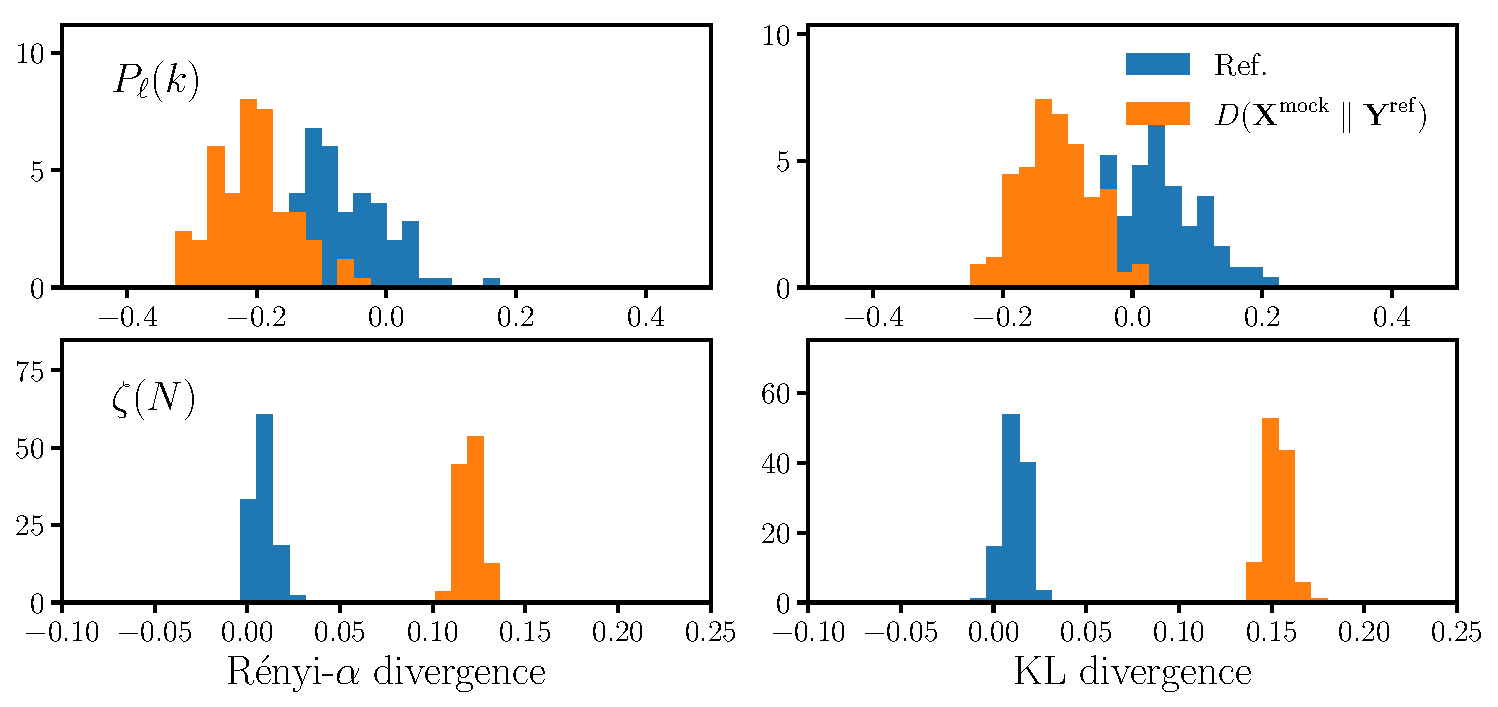
\includegraphics[width=0.9\textwidth]{figs/kNNdiverg_Gauss.pdf}
\caption{R\'enyi-$\alpha$ and KL divergence estimates, ($D_{R\alpha}$ and $D_{KL}$), 
between the mock data ${\bf X}^\mathrm{mock}$ and a reference sample 
${\bf Y}^\mathrm{ref}$ for the $P_\ell(k)$ (left) and $\zeta(N)$ (right) analyses.}
\label{fig:div_gauss}
\end{center}
\end{figure}


\begin{figure}
\begin{center}
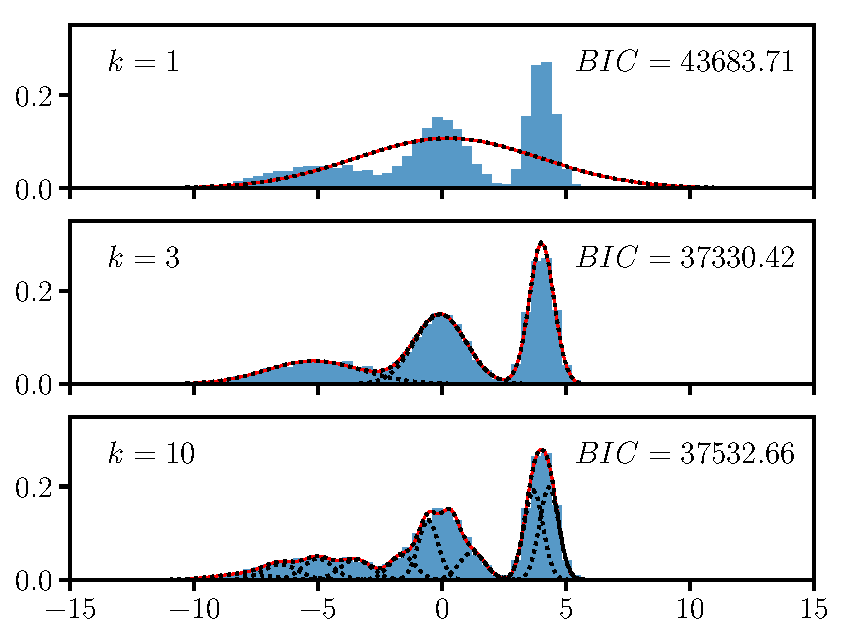
\includegraphics[width=0.75\textwidth]{figs/GMM_pedagog.pdf}
\caption{We use Gaussian mixture models with $k = 1$ (top), $3$, (middle), $10$ (bottom) 
    components to estimate the distribution of data (blue) drawn from three Gaussian distributions.
}
\label{fig:gmf_ped}
\end{center}
\end{figure}

\begin{figure}
\begin{center}
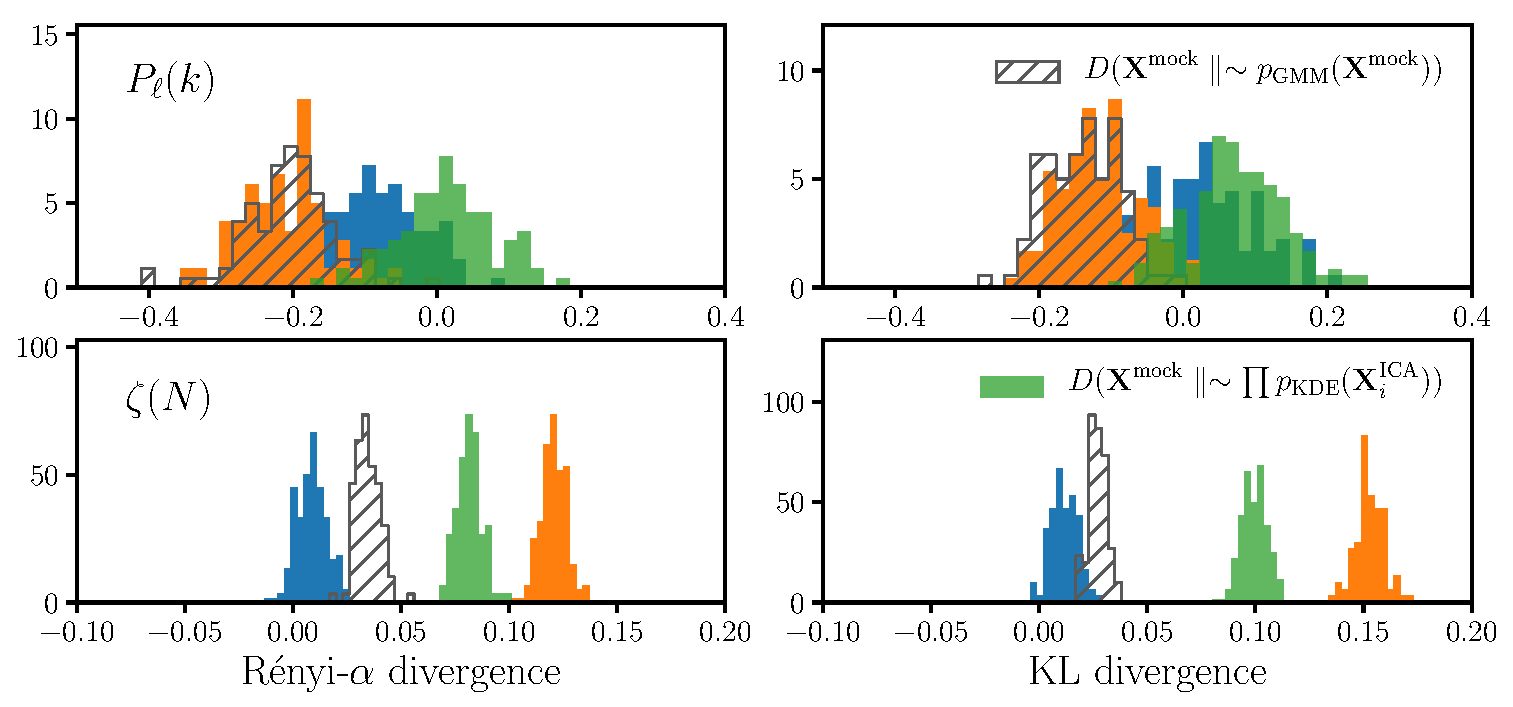
\includegraphics[width=0.9\textwidth]{figs/kNNdiverg_nonGauss.pdf}
\caption{}
\label{fig:div_nongauss}
\end{center}
\end{figure}

\begin{figure}
\begin{center}
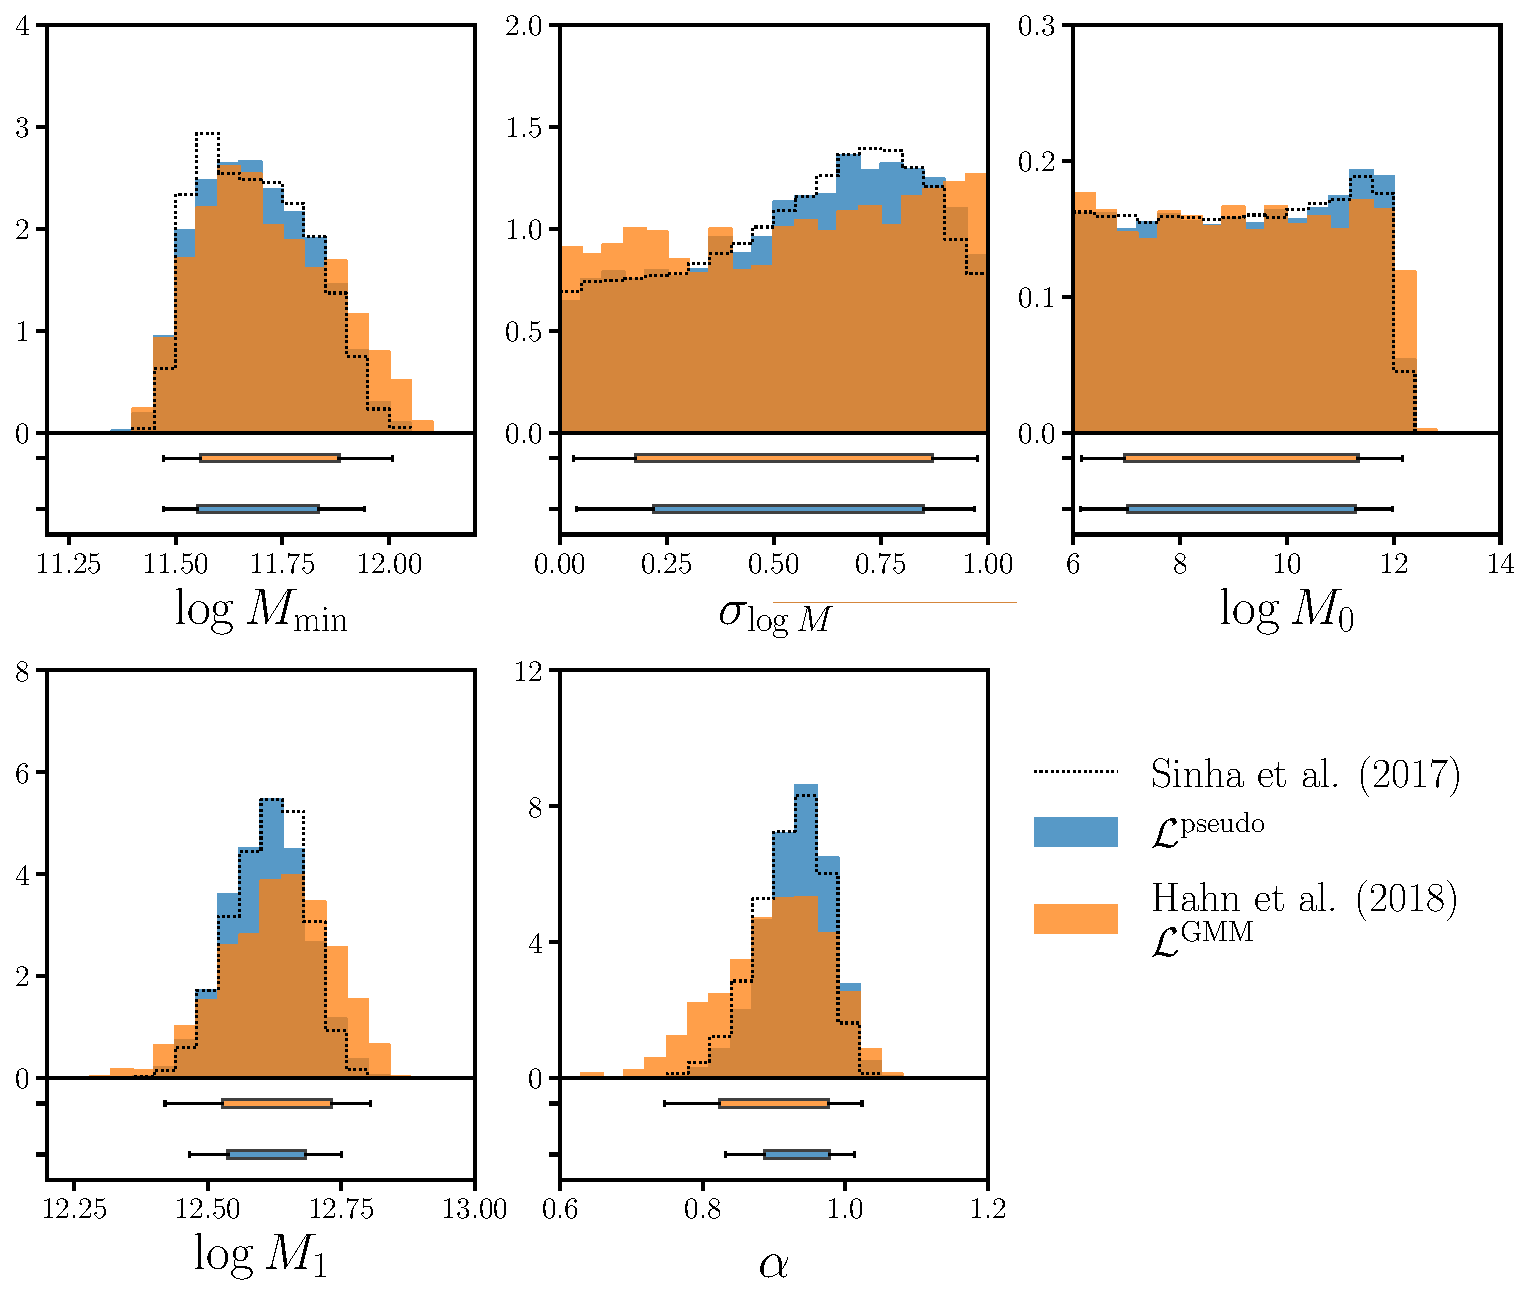
\includegraphics[width=\textwidth]{figs/Like_GMF_comparison.pdf}
\caption{}
\label{fig:gmf_like}
\end{center}
\end{figure}

\begin{figure}
\begin{center}
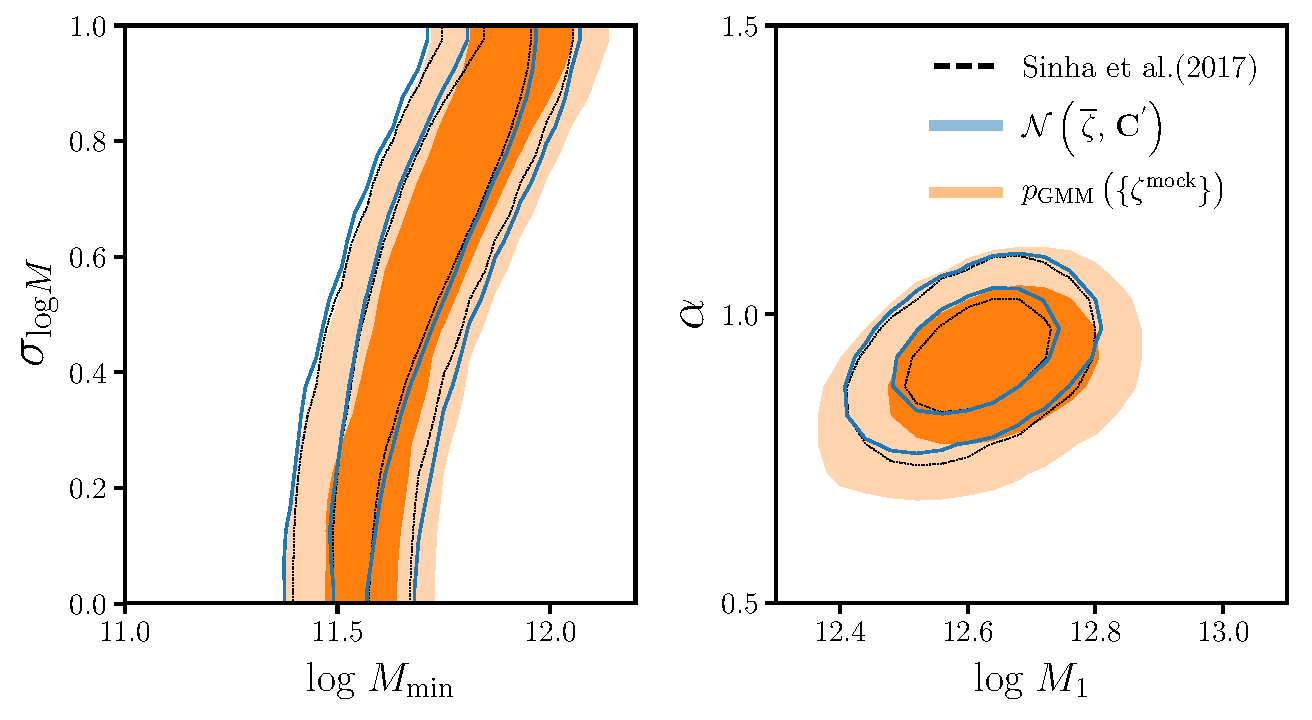
\includegraphics[width=0.9\textwidth]{figs/GMFcontours_manodeep.pdf}
\caption{}
\label{fig:gmf_contour}
\end{center}
\end{figure}

%%%%%%%%%%%%%%%%%%%%%%%%%%%%%%%%%%%%%%%%%%%%%%%%%%%%%%%%%%%%%%%
% Acknowledgements
%%%%%%%%%%%%%%%%%%%%%%%%%%%%%%%%%%%%%%%%%%%%%%%%%%%%%%%%%%%%%%%
\section*{Acknowledgements}
It's a pleasure to thank 
    Simone~Ferraro,
    David~W.~Hogg,
    Emmaneul~Schaan, 
    Roman~Scoccimarro
    Zachary~Slepian

\bibliographystyle{yahapj}
\bibliography{nongausslike}
\end{document}
